% =====================================================================
%  fig08 — Derivation pipeline (roadmap of the exact solution, Section 4)
%
%  A serpentine flowchart of the closed-form reduction in
%  "Type-specific catastrophe hazards in a two-type branching process".
%  Eight large stages take the two coupled backward equations to the
%  boxed exact finite-time probability S(t).
%
%    (1) autonomous type-2 solve  =>  G / z_2(t)      [type-2 INPUT]
%    (2) substitute into the type-1 (non-autonomous) Riccati
%    (3) shift by the long-time root   S = X + h
%    (4) linearise                     X = -Z'/Z
%    (5) change independent variable   t -> z_2,  Z = Phi(z_2)
%    (6) Gauss hypergeometric equation =>  2F1 basis U, V
%    (7) Wronskian initial condition   =>  K_U, K_V
%    (8) boxed exact S(t)                                [OUTPUT]
%
%  Schematic only: short phrases + key symbols, no fitted numerics.
%  Notation follows sections/03_autonomous.tex and 04_main_result.tex.
%
%  Vector schematic.  Build:  pdflatex fig08.tex   (-> fig08.pdf)
% =====================================================================
\documentclass[tikz,border=10pt]{standalone}

\usepackage[T1]{fontenc}
\usepackage{lmodern}          % match the paper's Latin Modern math
\usepackage{amsmath,amssymb,mathtools}
\usepackage{xcolor}

\usetikzlibrary{arrows.meta,positioning,calc,backgrounds,fit}

% ---- compact paper symbols ------------------------------------------
\newcommand{\Sh}{\widehat S}
\newcommand{\Gh}{\widehat G}
\newcommand{\qtwo}{\hat q_2}
\newcommand{\htF}{{}_2F_1}

% ---- palette (SHARED_CONVENTIONS.md) --------------------------------
\definecolor{type1}{HTML}{0072B2}   % type 1 / S  (primary blue)
\definecolor{type2}{HTML}{D55E00}   % type 2 / G  (vermillion)
\definecolor{ink}{HTML}{1A1C1F}     % near-black
\definecolor{inksoft}{HTML}{565B62} % secondary text
\definecolor{rule}{HTML}{E3E6EA}    % very light rules
\definecolor{okgreen}{HTML}{2E7D32} % result accent
\definecolor{type1fill}{HTML}{EAF2F9}
\definecolor{type1fillhi}{HTML}{DBEAF6}
\definecolor{type2fill}{HTML}{FBEEE5}
\definecolor{panelbg}{HTML}{FCFDFE}
\definecolor{cardfill}{HTML}{FFFFFF}

\begin{document}
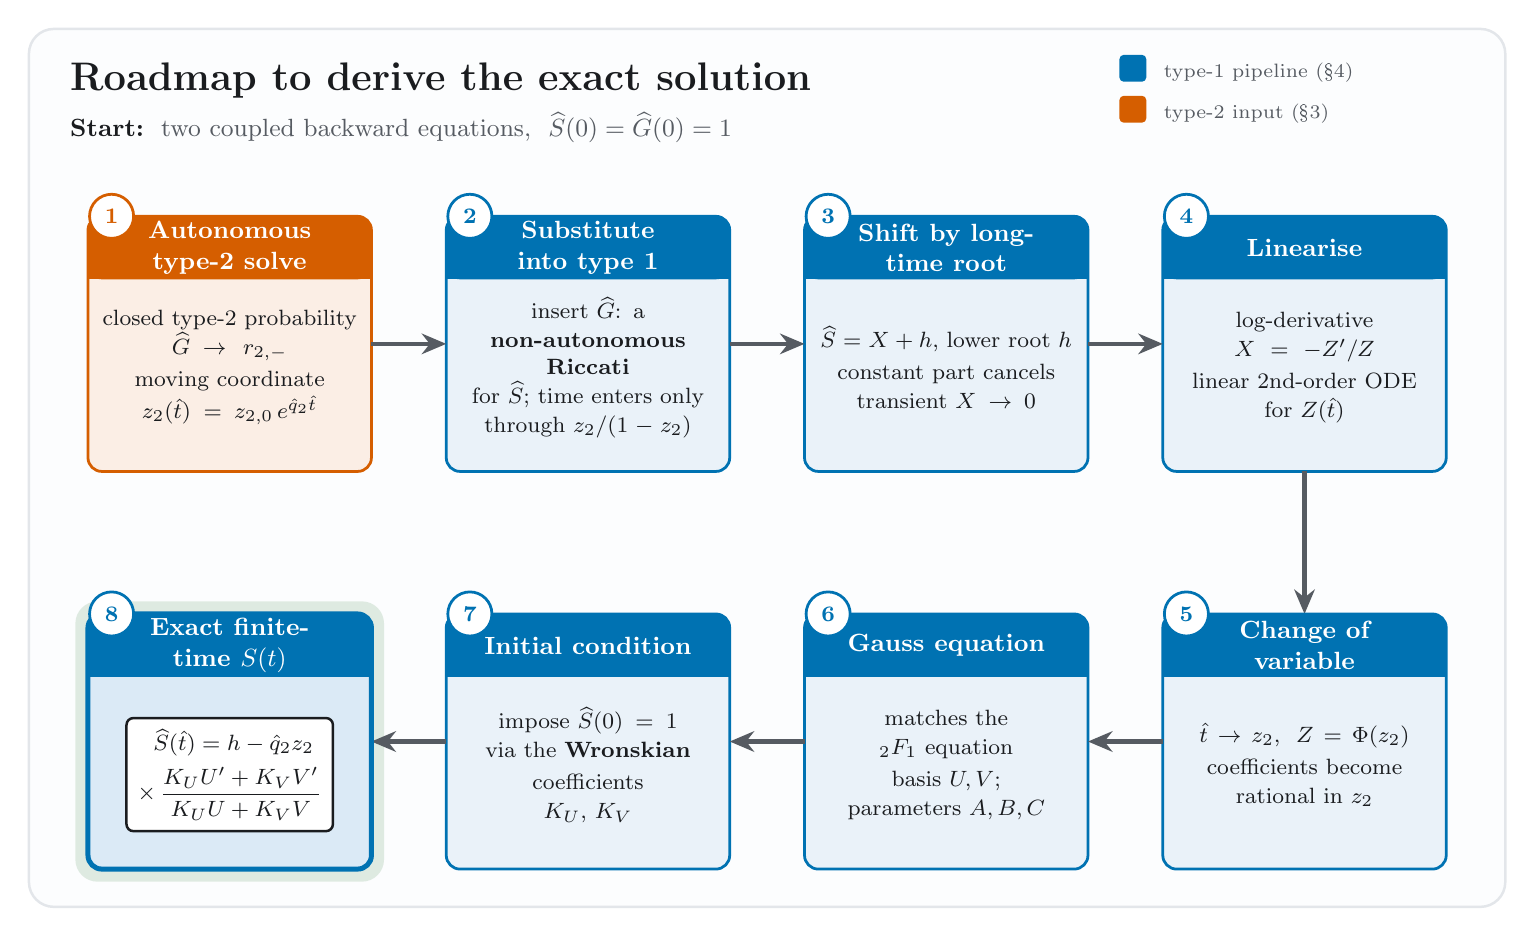
\begin{tikzpicture}[
    >={Stealth[length=3.1mm,width=2.6mm]},
    font=\normalsize,
    flow/.style={draw=inksoft,line width=1.5pt,-{Stealth[length=3.1mm,width=2.6mm]},
                 rounded corners=3pt},
  ]

% ---- card geometry (centimetres) ------------------------------------
\def\wh{1.80}        % card half-width
\def\hh{1.62}        % card half-height
\def\hdr{0.80}       % coloured header-strip height

% Row centres.  Serpentine: top row L->R (1..4), bottom row R->L (5..8).
\def\xA{0}   \def\xB{4.55} \def\xC{9.10} \def\xD{13.65}
\def\yT{2.15} \def\yB{-2.90}

% =====================================================================
%  Generic step card
%  #1 x  #2 y  #3 accent  #4 body-fill  #5 number  #6 title  #7 body
% =====================================================================
\newcommand{\stepcard}[7]{%
  % body + header
  \fill[#4,rounded corners=5pt] (#1-\wh,#2-\hh) rectangle (#1+\wh,#2+\hh);
  \fill[#3,rounded corners=5pt] (#1-\wh,#2+\hh-\hdr) rectangle (#1+\wh,#2+\hh);
  \fill[#3] (#1-\wh,#2+\hh-\hdr) rectangle (#1+\wh,#2+\hh-\hdr+0.14);% square header base
  \draw[#3,line width=1pt,rounded corners=5pt] (#1-\wh,#2-\hh) rectangle (#1+\wh,#2+\hh);
  % title
  \node[text=white,font=\bfseries\small,align=center,text width=3.15cm]
       at (#1,{#2+\hh-\hdr/2}) {#6};
  % body
  \node[text=ink,font=\footnotesize,align=center,text width=3.30cm]
       at (#1,{#2-0.30}) {#7};
  % number tab (drawn on the top-left corner)
  \node[circle,fill=white,draw=#3,line width=1pt,text=#3,
        font=\bfseries\footnotesize,minimum size=0.56cm,inner sep=0pt]
       at (#1-\wh+0.30,#2+\hh) {#5};
}

% =====================================================================
%  Background panel
% =====================================================================
\begin{scope}[on background layer]
  \fill[panelbg,rounded corners=9pt] (-2.55,-5.00) rectangle (16.20,6.15);
  \draw[rule,line width=0.9pt,rounded corners=9pt] (-2.55,-5.00) rectangle (16.20,6.15);
\end{scope}

% =====================================================================
%  Title block + legend
% =====================================================================
\node[ink,font=\Large\bfseries,anchor=west] at (-2.15,5.50)
     {Roadmap to derive the exact solution};
\node[inksoft,font=\small,anchor=west] at (-2.15,4.90)
     {\textbf{\textcolor{ink}{Start:}}\ \ two coupled backward equations,\ \ $\Sh(0)=\Gh(0)=1$};

% legend (top right)
\begin{scope}[shift={(11.30,5.58)}]
  \fill[type1,rounded corners=1.5pt] (0,-0.10) rectangle (0.34,0.24);
  \node[anchor=west,font=\scriptsize,text=inksoft] at (0.44,0.02) {type-1 pipeline (\S4)};
  \fill[type2,rounded corners=1.5pt] (0,-0.62) rectangle (0.34,-0.28);
  \node[anchor=west,font=\scriptsize,text=inksoft] at (0.44,-0.50) {type-2 input (\S3)};
\end{scope}

% =====================================================================
%  TOP ROW  (left to right):  1  ->  2  ->  3  ->  4
% =====================================================================
% (1) type-2 input -- vermillion
\stepcard{\xA}{\yT}{type2}{type2fill}{1}{Autonomous type-2 solve}
  {closed type-2 probability\\[1pt]
   $\Gh\!\to r_{2,-}$\\[2pt]
   moving coordinate\\[1pt]
   $z_2(\hat t)=z_{2,0}\,e^{\qtwo\hat t}$}

% (2) substitute -> Riccati
\stepcard{\xB}{\yT}{type1}{type1fill}{2}{Substitute into type~1}
  {insert $\Gh$: a\\[1pt]
   \textbf{non-autonomous Riccati}\\[1pt]
   for $\Sh$; time enters only\\[1pt]
   through $z_2/(1-z_2)$}

% (3) shift by long-time root
\stepcard{\xC}{\yT}{type1}{type1fill}{3}{Shift by long-time root}
  {$\Sh=X+h$, lower root $h$\\[2pt]
   constant part cancels\\[1pt]
   transient $X\to0$}

% (4) linearise
\stepcard{\xD}{\yT}{type1}{type1fill}{4}{Linearise}
  {log-derivative\\[1pt]
   $X=-Z'/Z$\\[2pt]
   linear 2nd-order ODE\\[1pt]
   for $Z(\hat t)$}

% top-row arrows
\draw[flow] (\xA+\wh,\yT) -- (\xB-\wh,\yT);
\draw[flow] (\xB+\wh,\yT) -- (\xC-\wh,\yT);
\draw[flow] (\xC+\wh,\yT) -- (\xD-\wh,\yT);

% =====================================================================
%  TURN DOWN  (right side):  4  ->  5
% =====================================================================
\draw[flow] (\xD,\yT-\hh) -- (\xD,\yB+\hh);

% =====================================================================
%  BOTTOM ROW  (right to left):  5  ->  6  ->  7  ->  8
% =====================================================================
% (5) change of variable
\stepcard{\xD}{\yB}{type1}{type1fill}{5}{Change of\\variable}
  {$\hat t\to z_2$,\ \ $Z=\Phi(z_2)$\\[2pt]
   coefficients become\\[1pt]
   rational in $z_2$}

% (6) Gauss equation -> 2F1
\stepcard{\xC}{\yB}{type1}{type1fill}{6}{Gauss equation}
  {matches the\\[1pt]
   ${}_2F_1$ equation\\[2pt]
   basis $U,V$;\\[1pt]
   parameters $A,B,C$}

% (7) Wronskian initial condition
\stepcard{\xB}{\yB}{type1}{type1fill}{7}{Initial condition}
  {impose $\Sh(0)=1$\\[1pt]
   via the \textbf{Wronskian}\\[2pt]
   coefficients\\[1pt]
   $K_U,\,K_V$}

% bottom-row arrows (leftward)
\draw[flow] (\xD-\wh,\yB) -- (\xC+\wh,\yB);
\draw[flow] (\xC-\wh,\yB) -- (\xB+\wh,\yB);
\draw[flow] (\xB-\wh,\yB) -- (\xA+\wh,\yB);

% =====================================================================
%  (8) OUTPUT — boxed exact S(t)  (highlighted)
% =====================================================================
% soft halo behind the output card
\begin{scope}[on background layer]
  \fill[okgreen,opacity=0.14,rounded corners=8pt]
        (\xA-\wh-0.16,\yB-\hh-0.16) rectangle (\xA+\wh+0.16,\yB+\hh+0.16);
\end{scope}
% card body + emphasised frame
\fill[type1fillhi,rounded corners=5pt] (\xA-\wh,\yB-\hh) rectangle (\xA+\wh,\yB+\hh);
\fill[type1,rounded corners=5pt] (\xA-\wh,\yB+\hh-\hdr) rectangle (\xA+\wh,\yB+\hh);
\fill[type1] (\xA-\wh,\yB+\hh-\hdr) rectangle (\xA+\wh,\yB+\hh-\hdr+0.14);
\draw[type1,line width=1.8pt,rounded corners=5pt]
     (\xA-\wh,\yB-\hh) rectangle (\xA+\wh,\yB+\hh);
\node[text=white,font=\bfseries\small,align=center,text width=3.15cm]
     at (\xA,{\yB+\hh-\hdr/2}) {Exact finite-time $S(t)$};
% boxed formula (echoes the boxed equation in the paper)
\node[draw=ink,line width=0.9pt,rounded corners=2.5pt,fill=cardfill,
      inner xsep=4pt,inner ysep=4pt,text=ink,font=\footnotesize,align=center]
     at (\xA,\yB-0.42)
     {$\displaystyle \Sh(\hat t)=h-\qtwo z_2\!\!$\\[3pt]
      $\displaystyle \times\,\frac{K_U U'+K_V V'}{K_U U+K_V V}$};
% number tab
\node[circle,fill=white,draw=type1,line width=1pt,text=type1,
      font=\bfseries\footnotesize,minimum size=0.56cm,inner sep=0pt]
     at (\xA-\wh+0.30,\yB+\hh) {8};

\end{tikzpicture}
\end{document}
